\documentclass[10pt]{standalone}
\usepackage[sc]{mathpazo}
\usepackage{commands}
\renewcommand{\phi}{\varphi}

\begin{document}
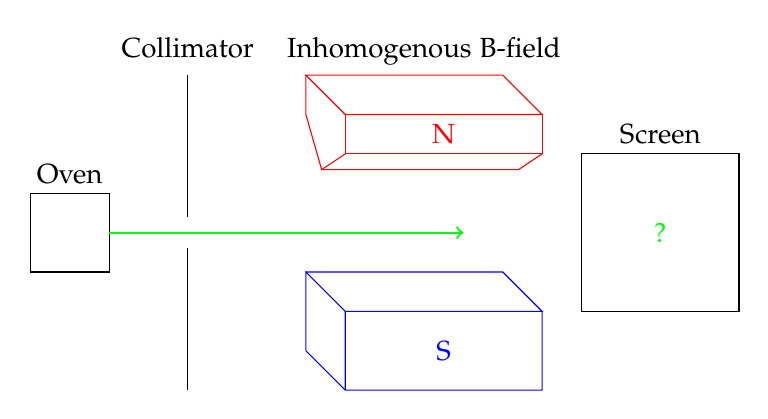
\begin{tikzpicture}
    \draw[] (-0.5, -0.5) -- (0.5, -0.5) -- (0.5, 0.5) -- (-0.5, 0.5) -- cycle;
    \node[above] at (0, 0.5) {Oven};
    \draw[] (1.5, 2) -- (1.5, 0.2);
    \draw[] (1.5, -2) -- (1.5, -0.2);
    \node[above] at (1.5, 2.1) {Collimator};
    \draw[green, thick, ->] (0.5, 0) -- (5, 0); 
    \draw[red] (3, 2) -- (3.5, 1.5) -- (6, 1.5) -- (5.5, 2) -- cycle;
    \draw[red] (3.5, 1.5) -- (3.5, 1) -- (6, 1) -- (6, 1.5);
    \draw[red] (3, 2) -- (3, 1.5) -- (3.2, 0.8) -- (3.5, 1);
    \draw[red] (3.2, 0.8) -- (5.7, 0.8) -- (6, 1);
    \node[red] at (4.75, 1.25) {N};
    \draw[blue] (3, -1.5) --(3.5, -2) -- (6, -2) -- (6, -1);
    \draw[blue] (3, -1.5) -- (3, -0.5) -- (3.5, -1) -- (3.5, -2);
    \draw[blue] (3.5, -1) -- (6, -1) -- (5.5, -0.5) -- (3, -0.5);
    \node[blue] at (4.75, -1.5) {S};
    \node[above] at (4.5, 2) {Inhomogenous B-field};
    \draw[] (6.5, 1) -- (8.5, 1) -- (8.5, -1) -- (6.5, -1) -- cycle;
    \node[above] at (7.5, 1) {Screen};
    \node[green] at (7.5, 0) {?};

\end{tikzpicture}
\end{document}